\documentclass[a4paper,12pt]{article}
\usepackage[utf8]{inputenc}
\usepackage[T1]{fontenc}
\usepackage[french]{babel}
\usepackage{graphicx}      
\usepackage{geometry}       
\usepackage{amsmath, amssymb, amsthm} 
\usepackage{listings}       
\usepackage{xcolor}       
\usepackage{hyperref}      
\usepackage{float}          
\usepackage{fancyhdr}      
\usepackage{tikz}           
\geometry{hmargin=2.5cm,vmargin=2.5cm}
\setlength{\parskip}{1em} 

\definecolor{codegreen}{rgb}{0,0.6,0}
\definecolor{codegray}{rgb}{0.5,0.5,0.5}
\definecolor{codepurple}{rgb}{0.58,0,0.82}
\definecolor{backcolour}{rgb}{0.95,0.95,0.92}

\lstdefinestyle{styleCpp}{
    backgroundcolor=\color{backcolour},   
    commentstyle=\color{codegreen},
    keywordstyle=\color{magenta},
    numberstyle=\tiny\color{codegray},
    stringstyle=\color{codepurple},
    basicstyle=\ttfamily\small,
    breakatwhitespace=false,         
    breaklines=true,                 
    captionpos=b,                    
    keepspaces=true,                 
    numbers=left,                    
    numbersep=5pt,                  
    showspaces=false,                
    showstringspaces=false,
    showtabs=false,                  
    tabsize=4,
    language=C++
}

\pagestyle{fancy}
\fancyhf{}
\rhead{Projet Simulation Chaleur}
\lhead{ENSIIE 2025-2026}
\cfoot{\thepage}


\begin{document}


\begin{titlepage}
    \centering
    \vspace*{2cm}
    \includegraphics[width=0.9\textwidth]{ensiie_logo_fx_RVB_0.png} 
    
    \vspace{2cm}
    {\Huge \textbf{Rapport de Projet PAP}}\\
    \vspace{0.5cm}
    {\huge \textit{Résolution Numérique de l'Équation de la Chaleur}}\\
    \vspace{1.5cm}
    
    \textbf{\Large ENSIIE -- 2e Année}\\
    \textbf{\large Janvier 2026}
    
    \vspace{3cm}
    \textbf{Auteurs :}\\
    \Large GRASSIAN Arnaud\\
    \Large RHOUDDAL Saad
    
    \vspace{2cm}
    \date{\today}
\end{titlepage}

\tableofcontents
\newpage



\section{Présentation du Problème Physique}


L'objectif de ce projet est de simuler la diffusion thermique au sein de différents matériaux. Ce phénomène physique est décrit par une équation aux dérivées partielles (EDP) : \textbf{l'équation de la chaleur}.

\subsection{Formulation Mathématique}
L'équation régit l'évolution de la température $u$ en fonction du temps $t$ et de l'espace.

\subsubsection{Cas 1D : La Barre}
Pour une barre unidimensionnelle de longueur $L$, l'équation s'écrit :
\begin{equation}
    \frac{\partial u}{\partial t} = \alpha \frac{\partial^2 u}{\partial x^2} + F(x,t)
\end{equation}
Les termes sont définis comme suit :
\begin{itemize}
    \item $u(x,t)$ : Température au point $x$ à l'instant $t$ (en Kelvin).
    \item $\alpha$ : Diffusivité thermique du matériau, définie par $\alpha = \frac{\lambda}{\rho c}$.
    \item $F(x,t)$ : Terme source représentant un apport externe de chaleur (normalisé par $\rho c$).
\end{itemize}

\subsubsection{Cas 2D : La Plaque}
Pour une plaque bidimensionnelle, la diffusion s'opère selon les axes $x$ et $y$. L'équation devient :
\begin{equation}
    \frac{\partial u}{\partial t} = \alpha \left( \frac{\partial^2 u}{\partial x^2} + \frac{\partial^2 u}{\partial y^2} \right) + F(x,y,t)
\end{equation}

\subsection{Nécessité de la Résolution Numérique}
Les équations aux dérivées partielles (EDP) présentées ci-dessus admettent rarement des solutions analytiques simples, en particulier lorsque le terme source $F$ est complexe ou que les conditions aux bords sont mixtes.

Pour contourner cette difficulté, nous utilisons des \textbf{méthodes numériques}. L'approche consiste à discrétiser le domaine continu (espace et temps) pour transformer l'équation différentielle en un système d'équations algébriques. Ce système peut alors être résolu itérativement par un ordinateur.








\section{Le Sujet du Projet}
Nous devons simuler cette équation sur un domaine borné $[0, L]^d$ (avec $d=1$ ou $d=2$) sur une durée $t \in [0, t_{max}]$. 
Les conditions initiales imposent une température uniforme $u(0, x) = u_0 = 13^\circ C$.

\subsection{Conditions aux Limites (Bords)}
Il faut définir ce qui se passe aux frontières du domaine. Le sujet impose des conditions  :

\subsection{Condition de Dirichlet}
Elle impose une valeur fixe à la température sur le bord.
$$ u(t, L) = u_{fixe} $$
Physiquement, cela signifie que le bord est mis en contact avec un thermostat parfait qui maintient la température constante.

\subsection{Condition de Neumann}
La condition de Neumann homogène impose que le flux de chaleur traversant la paroi soit nul, ce qui correspond physiquement à une isolation parfaite (paroi adiabatique.

Dans notre géométrie cartésienne alignée avec les axes $(Ox, Oy)$, cette condition se traduit simplement par l'annulation de la dérivée partielle par rapport à la variable perpendiculaire au bord :

\begin{itemize}
    \item \textbf{Sur le bord vertical gauche ($x=0$)} : La variation de température doit être nulle selon l'axe $x$.
    $$ \frac{\partial u}{\partial x}(0, t) = 0 $$
    
    \item \textbf{Sur le bord horizontal inférieur ($y=0$)} : La variation de température doit être nulle selon l'axe $y$ (cas 2D uniquement).
    $$ \frac{\partial u}{\partial y}(x, 0, t) = 0 $$
\end{itemize}

Cette simplification est possible car nos bords sont strictement parallèles aux axes du repère.


\section{La Méthode des Différences Finies}

Pour résoudre numériquement l'équation, nous transformons le domaine continu en une grille discrète. Cette opération se décompose en deux aspects :

\begin{itemize}
    \item \textbf{Discrétisation temporelle :} L'intervalle de temps $[0, t_{max}]$ est divisé en pas constants $\Delta t$. On cherche la solution aux instants $t_n = n \cdot \Delta t$.
    \item \textbf{Discrétisation spatiale :} Le matériau est divisé en cellules.
    \begin{itemize}
        \item En 1D : Un segment de pas $\Delta x$.
        \item En 2D : Un maillage rectangulaire de pas $\Delta x$ et $\Delta y$.
    \end{itemize}
\end{itemize}



\subsection{Approximations et Schéma Numérique}

Pour transformer l'EDP en un système algébrique résoluble, nous remplaçons les dérivées par des différences finies basées sur les développements de Taylor.

\subsubsection{Discrétisation Temporelle : Le Choix de l'Implicite}
Deux approches principales existent pour la dérivée temporelle :
\begin{itemize}
    \item \textbf{Schéma Explicite} : Simple à calculer mais conditionnellement stable (nécessite un $\Delta t$ très petit).
    \item \textbf{Schéma Implicite} : Nécessite la résolution d'un système linéaire mais est \textbf{inconditionnellement stable}.
\end{itemize}

En accord avec le sujet, nous avons choisi le schéma implicite . L'approximation est donc :
\begin{equation}
    \frac{\partial u}{\partial t} \approx \frac{u^{n+1} - u^n}{\Delta t}
\end{equation}

\subsubsection{Discrétisation Spatiale (Laplacien)}
Les dérivées spatiales sont approchées par des différences finies centrées.

\textbf{Cas 1D (Barre) :} La dérivée seconde utilise le point $i$ et ses deux voisins :
\begin{equation}
    \frac{\partial^2 u}{\partial x^2} \approx \frac{u_{i-1} - 2u_i + u_{i+1}}{\Delta x^2}
\end{equation}

\textbf{Cas 2D (Plaque) :} Le Laplacien somme les dérivées dans les deux directions ($x$ et $y$), impliquant le point $(i,j)$ et ses quatre voisins :
\begin{equation}
    \Delta u \approx \frac{u_{i-1,j} - 2u_{i,j} + u_{i+1,j}}{\Delta x^2} + \frac{u_{i,j-1} - 2u_{i,j} + u_{i,j+1}}{\Delta y^2}
\end{equation}









\section{Résolution du Cas 1D (La Barre)}

\subsection{Discrétisation de l'Équation}
En 1D, le schéma implicite donne :
$$ \frac{u_i^{n+1} - u_i^n}{\Delta t} = \alpha \frac{u_{i+1}^{n+1} - 2u_i^{n+1} + u_{i-1}^{n+1}}{\Delta x^2} + S_i $$


Où $S_i$ représente le terme source normalisé par les propriétés thermiques du matériau au point $x_i$. D'après l'équation (1) du sujet, il est défini par :

\begin{equation}
    S_i = \frac{F(x_i, t)}{\rho c}
\end{equation}

Avec :
\begin{itemize}
    \item $F(x_i, t)$ : La valeur de la source de chaleur imposée (en $W \cdot m^{-3}$ ou unité arbitraire du sujet) au nœud $i$.
    \item $\rho$ : La masse volumique du matériau ($kg \cdot m^{-3}$).
    \item $c$ : La chaleur massique ($J \cdot kg^{-1} \cdot K^{-1}$).
\end{itemize}\\



En posant $r = \frac{\alpha \Delta t}{\Delta x^2}$, on peut réarranger les termes pour isoler les inconnues (à l'instant $n+1$) à gauche :
$$ -r u_{i-1}^{n+1} + (1 + 2r) u_i^{n+1} - r u_{i+1}^{n+1} = u_i^n + \Delta t \cdot S_i $$

Ceci est un système linéaire de la forme $A U = B$, où $A$ est une matrice tridiagonale (=matrice dont tous les coefficients qui ne sont ni sur la diagonale principale, ni sur la diagonale juste au-dessus, ni celle juste en dessous, sont nuls).

\subsection{Algorithme de Résolution : Thomas}
Pour résoudre ce système $Ax=b$, utiliser une méthode générique comme le Pivot de Gauss ($O(N^3)$) serait beaucoup trop lent pour $N=1001$. Heureusement, la matrice $A$ a une structure très particulière : elle n'a des zéros partout sauf sur la diagonale principale et ses deux voisines.

L'algorithme de Thomas (TDMA - TriDiagonal Matrix Algorithm) est une simplification de la décomposition LU optimisée pour ce cas. Il se déroule en deux étapes et a une complexité en $O(N)$, ce qui est optimal.

\subsubsection{Étape 1 : Élimination}
On élimine la diagonale inférieure pour transformer la matrice en triangulaire supérieure. On modifie les coefficients $c_i$ (diagonale sup) et $d_i$ (second membre) :
$$ c'_i = \frac{c_i}{b_i - a_i c'_{i-1}} $$
$$ d'_i = \frac{d_i - a_i d'_{i-1}}{b_i - a_i c'_{i-1}} $$

\subsubsection{Étape 2 : Substitution}
On remonte du dernier point vers le premier pour trouver la solution :
$$ u_N = d'_N $$
$$ u_i = d'_i - c'_i u_{i+1} $$

\subsection{Traitement des Conditions aux Limites}
\subsubsection{Neumann en $x=0$}



L'application de la condition de Neumann ($\frac{\partial u}{\partial x} = 0$) au point d'indice $i=0$ pose une difficulté particulière. En effet, le schéma des différences finies fait normalement intervenir le point de gauche ($i-1$), or le point d'indice $-1$ n'existe pas physiquement : il est hors de la barre.

Pour résoudre ce problème tout en conservant une précision d'ordre 2, nous utilisons la technique du \textbf{point fantôme}.

\paragraph{1. Introduction du point virtuel}
Nous imaginons un point virtuel $u_{-1}$ situé juste à l'extérieur du domaine, à une distance $\Delta x$ du bord. Nous appliquons ensuite l'approximation de la dérivée centrée en $x=0$ :
\begin{equation}
    \frac{\partial u}{\partial x}(0) \approx \frac{u_{1} - u_{-1}}{2\Delta x} = 0
\end{equation}

\paragraph{2. Relation de symétrie}
L'équation ci-dessus implique directement que la température virtuelle doit être symétrique par rapport au bord :
\begin{equation}
    u_{1} - u_{-1} = 0 \quad \Longrightarrow \quad u_{-1} = u_{1}
\end{equation}
Cela signifie que, pour respecter l'isolation thermique, la température virtuelle à gauche doit être égale à la température réelle à droite immédiate du bord.

\paragraph{3. Réinjection dans le schéma numérique}
L'équation générale discrétisée pour une cellule quelconque $i$ est :
$$ -r u_{i-1} + (1 + 2r) u_i - r u_{i+1} = u_i^n + \Delta t S_i $$
En l'appliquant à $i=0$ et en remplaçant l'inconnue $u_{-1}$ par $u_{1}$, l'équation devient :
$$ -r (u_{1}) + (1 + 2r) u_0 - r u_{1} = u_0^n + \Delta t S_0 $$

\paragraph{4. Résultat Final}
En regroupant les termes en $u_{1}$, nous obtenons la nouvelle équation pour la première ligne de notre système matriciel :
\begin{equation}
    (1 + 2r) u_0 - 2r u_{1} = u_0^n + \Delta t S_0
\end{equation}
Cette manipulation est essentielle car elle permet d'éliminer l'inconnue impossible $u_{-1}$ tout en \textbf{préservant la structure tridiagonale} de la matrice (seuls les coefficients de la première ligne changent). Cela nous permet d'utiliser l'algorithme de Thomas sans modification.





























\section{Résolution du Cas 2D (La Plaque)}

\subsection{Complexité du passage à la 2D}
En 2D, l'équation implicite relie 5 points de la grille (le point central et ses 4 voisins Haut, Bas, Gauche, Droite). La matrice résultante n'est plus tridiagonale mais "pentadiagonale avec des trous" (matrice carrée qui ne contient que 5 diagonales non nullesdon). L'inversion directe de cette matrice est très coûteuse.




\begin{equation}
A = 
\begin{pmatrix}
d & a & 0 & \dots & 0 & b & 0 & \dots & 0 \\
a & d & a & 0 & \dots & 0 & b & \ddots & \vdots \\
0 & a & d & a & \ddots & & \ddots & \ddots & 0 \\
\vdots & 0 & a & \ddots & \ddots & \ddots & & \ddots & b \\
0 & \vdots & \ddots & \ddots & d & \ddots & \ddots & \vdots & 0 \\
b & 0 & & \ddots & \ddots & \ddots & a & 0 & \vdots \\
0 & b & \ddots & & \ddots & a & d & a & 0 \\
\vdots & \ddots & \ddots & 0 & \dots & 0 & a & d & a \\
0 & \dots & 0 & b & 0 & \dots & 0 & a & d
\end{pmatrix}
\end{equation}

Où :
\begin{itemize}
    \item $d$ : Diagonale principale (point central $(i,j)$).
    \item $a$ : Diagonales adjacentes (voisins gauche/droite $(i\pm 1, j)$).
    \item $b$ : Diagonales éloignées (voisins haut/bas $(i, j\pm 1)$).
    \item Les zones remplies de $0$ et de $\dots$ représentent les "trous".
\end{itemize}





\subsection{La Méthode ADI (Alternating Direction Implicit)}
Pour contourner ce problème, nous utilisons la méthode ADI. L'idée est de diviser le pas de temps en deux demi-étapes :

\subsubsection{Demi-pas 1 : Implicite en X, Explicite en Y}
On passe du temps $t$ à $t + \Delta t/2$.
On traite la diffusion selon $X$ de manière implicite (inconnues à gauche) et la diffusion selon $Y$ de manière explicite (connues à droite).
$$ \text{Termes en } X^{n+1/2} = \text{Termes en } Y^n + \text{Termes en } X^n $$
Cela revient à résoudre $N$ systèmes tridiagonaux indépendants (un pour chaque ligne de la grille). On peut donc réutiliser l'algorithme de Thomas.

\subsubsection{Demi-pas 2 : Explicite en X, Implicite en Y}
On passe du temps $t + \Delta t/2$ à $t + \Delta t$.
On inverse les rôles : $X$ devient explicite et $Y$ implicite.
$$ \text{Termes en } Y^{n+1} = \text{Termes en } X^{n+1/2} + \text{Termes en } Y^{n+1/2} $$
Cela revient à résoudre $N$ systèmes tridiagonaux indépendants (un pour chaque colonne).

\section{Avantages de l'approche}
\begin{itemize}
    \item \textbf{Rapidité} : On ne résout que des systèmes tridiagonaux ($O(N)$) au lieu d'un énorme système 2D.
    \item \textbf{Stabilité} : La méthode est stable(sans condition).
    \item \textbf{Précision} : L'ordre de précision est de 2 en temps et en espace.
\end{itemize}






\section{Organisation du Code}

Le code est séparé en trois parties logiques : la définition physique (Matériau), la résolution mathématique (Solveurs) et l'interface graphique (SDL).






\begin{figure}[H]
    \centering
    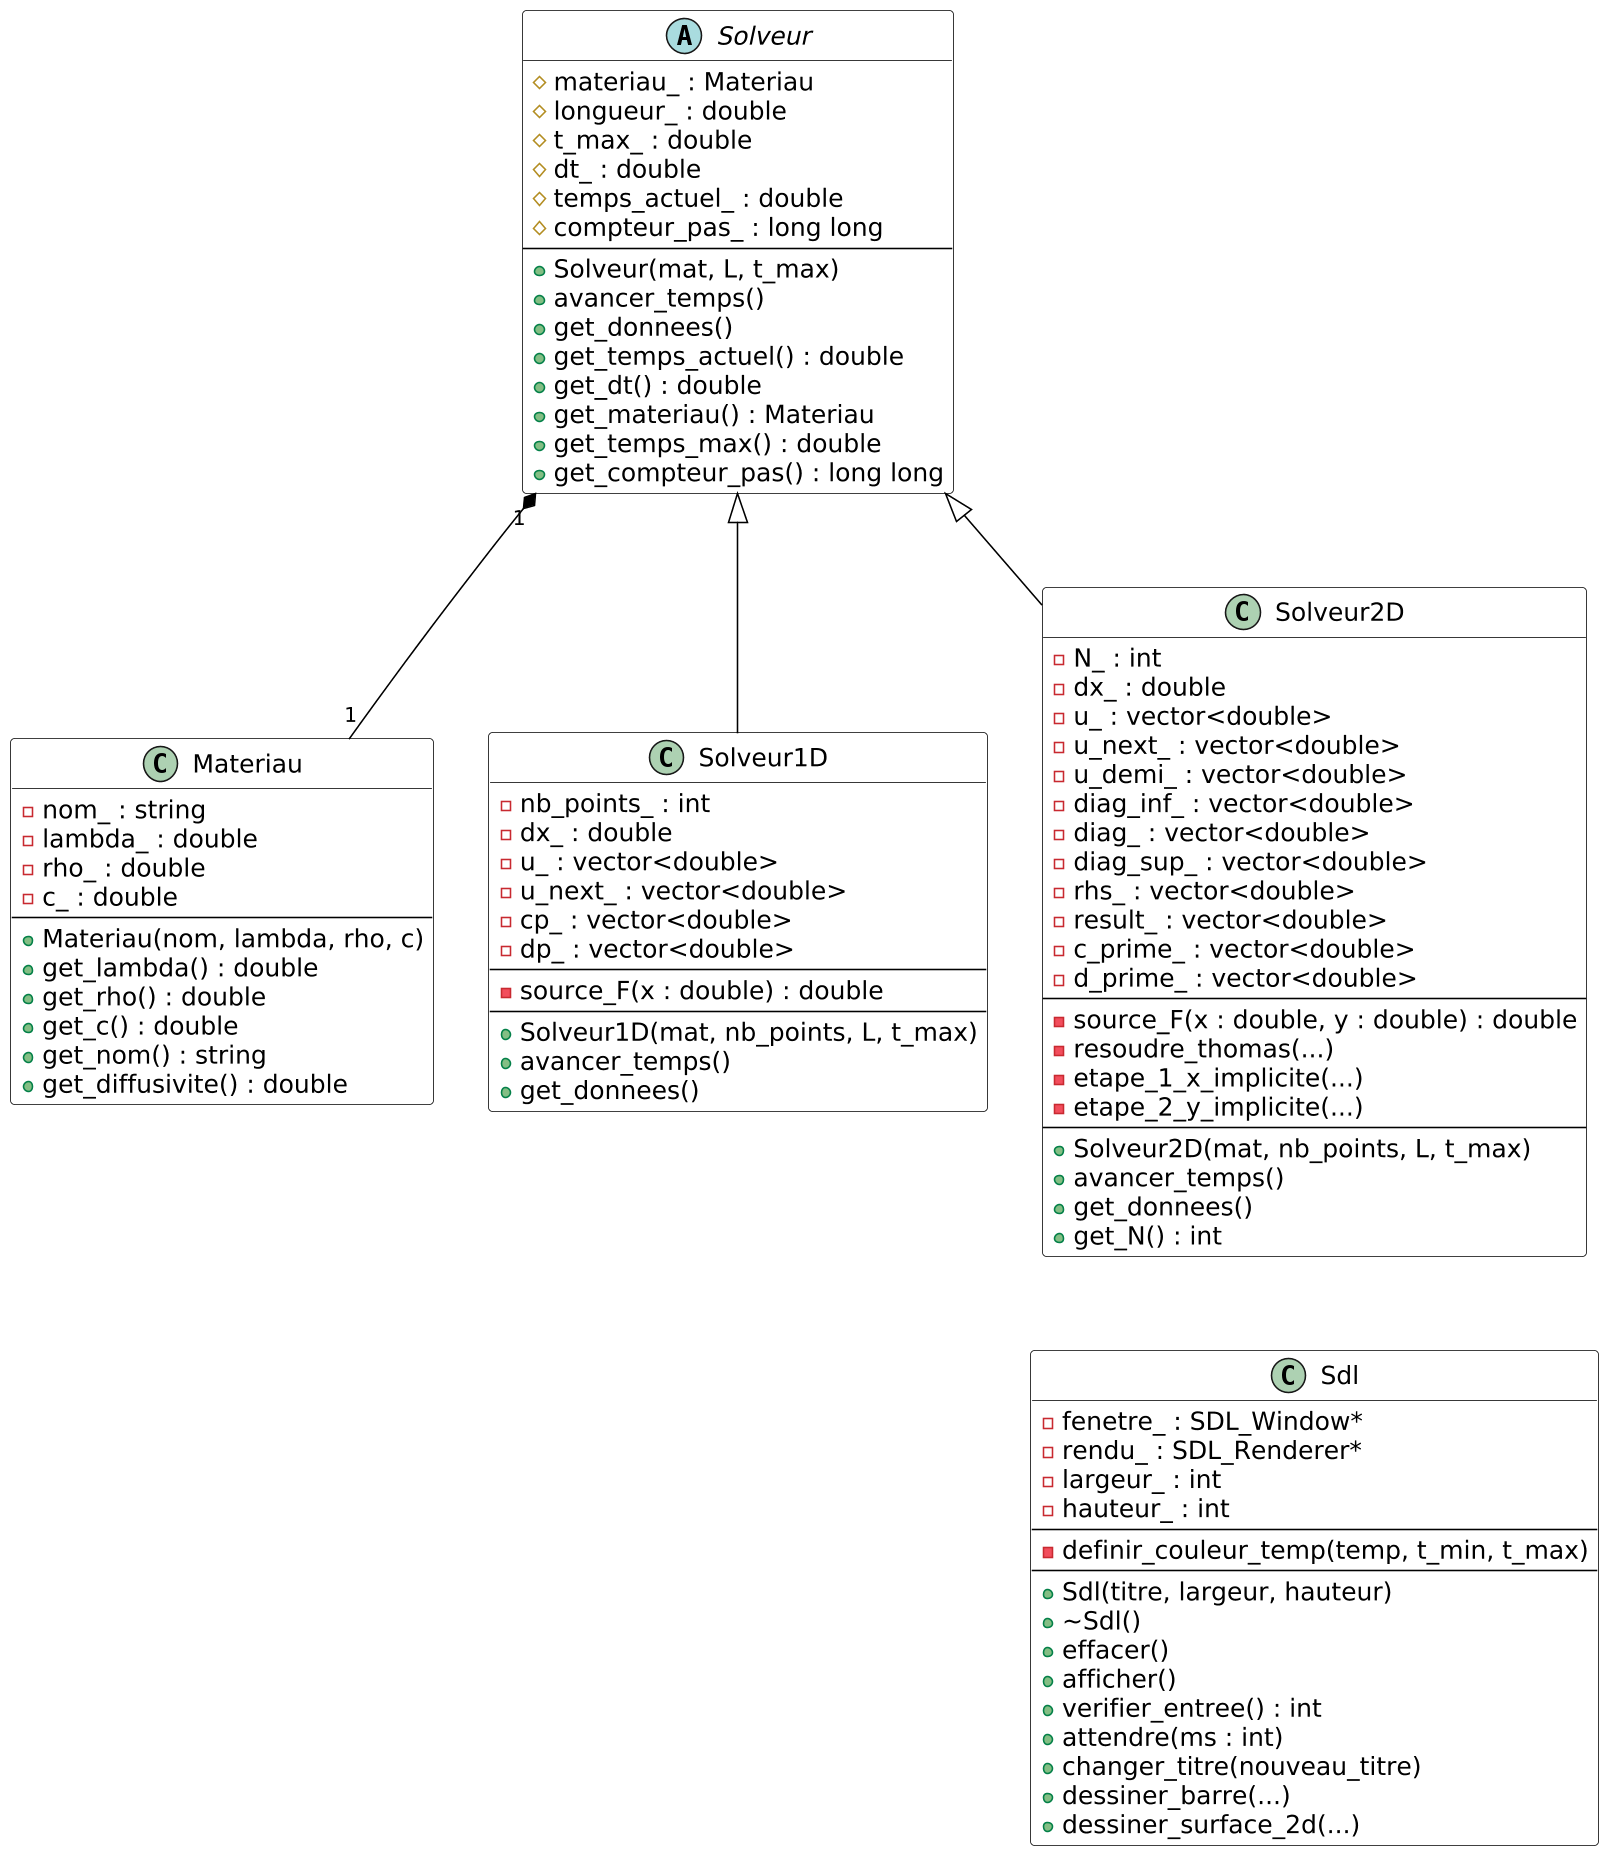
\includegraphics[width=1.1\textwidth]{uml.png}
    \caption{Diagramme UML de l'architecture du projet}
    \label{fig:uml}
    \vspace{0.2cm}
    \small
    \textit{Note : Pour la signification détaillée des modificateurs d'accès, voir la légende sur \href{https://commons.wikimedia.org/wiki/File:UML_class_diagram_with_access_modifiers.svg}{Wikimedia Commons}.}
\end{figure}

\textit{Note : Par souci de lisibilité, la structure de données (comme \texttt{EtapeLog}) n'est pas représentée (elle ne possède que 3 nombres).}













Voici une description détaillée de chaque composant et de leurs interactions.





















\subsection{Gestion des Données Physiques : \texttt{materiau.h}}
La classe \texttt{Materiau} agit comme un conteneur de données.

\begin{itemize}
    \item \textbf{Rôle :} Elle encapsule les constantes physiques propres à chaque matériau : la conductivité thermique $\lambda$, la masse volumique $\rho$, et la chaleur massique $c$.
    \item \textbf{Fonctionnalité clé :} Elle calcule automatiquement la diffusivité thermique $\alpha = \frac{\lambda}{\rho c}$ via la méthode \texttt{get\_diffusivite()}.
    
\end{itemize}

\subsection{Le Cœur du Calcul : La Hiérarchie \texttt{Solveur}}
Pour traiter indifféremment les cas 1D et 2D, nous avons utilisé l'héritage et le polymorphisme.


\subsubsection{La Classe Abstraite \texttt{Solveur}}
Définie dans \texttt{solveur.h}, c'est la classe "parent".
\begin{itemize}
    \item Elle gère les attributs communs : le temps actuel, le pas de temps $\Delta t$, la longueur $L$ et l'objet \texttt{Materiau}.
    \item Elle déclare une méthode virtuelle pure \texttt{avancer\_temps()}. Cela signifie que la classe \texttt{Solveur} ne sait pas comment résoudre l'équation, mais elle oblige ses "enfants" (1D et 2D) à fournir cette fonctionnalité.
\end{itemize}

\subsubsection{Le \texttt{Solveur1D} (La Barre)}
C'est la classe spécialisée pour la simulation unidimensionnelle.
\begin{itemize}
    \item \textbf{Stockage :} Elle utilise des vecteurs \texttt{std::vector<double>} pour stocker la température $u$ le long de la ligne.
    \item \textbf{Algorithme :} Sa méthode \texttt{avancer\_temps()} construit les trois diagonales de la matrice implicite et le membre de droite (avec la source de chaleur $F$).
    \item \textbf{Résolution :} Elle implémente l'algorithme de Thomas directement pour inverser la matrice tridiagonale en une seule passe.
\end{itemize}

\subsubsection{Le \texttt{Solveur2D} (La Plaque)}
C'est la classe la plus complexe, spécialisée pour la surface carrée.
\begin{itemize}
    \item \textbf{Découpage en sous-étapes :} Pour plus de lisibilité, la méthode \texttt{avancer\_temps()} appelle deux sous-méthodes correspondant à la méthode ADI :
    \begin{enumerate}
        \item \texttt{etape\_1\_x\_implicite} : Résout la diffusion en $x$ (ligne par ligne).
        \item \texttt{etape\_2\_y\_implicite} : Résout la diffusion en $y$ (colonne par colonne).
    \end{enumerate}
    \item \textbf{Optimisation Mémoire :} Contrairement à une approche naïve qui recréerait des vecteurs à chaque tour de boucle, le \texttt{Solveur2D} pré-alloue tous ses vecteurs de travail (diagonales, vecteurs intermédiaires pour Thomas) dans son constructeur. Cela évite des milliers d'allocations mémoire inutiles par seconde.
\end{itemize}











\subsection{L'Interface Graphique : \texttt{Sdl} (\texttt{sdl\_gestion.h})}
La classe \texttt{Sdl} agit comme une interface simplifiée pour la bibliothèque SDL2. Ses principales caractéristiques sont :

\begin{itemize} \item \textbf{Séparation de l'affichage :} La classe se concentre uniquement sur le visuel. Elle convertit les données brutes (températures) en couleurs, sans avoir besoin de comprendre la logique physique de la simulation. \item \textbf{Fluidité d'affichage :} Pour garantir une animation rapide même avec un grand nombre de points, la méthode \texttt{dessiner\_surface\_2d} est optimisée. Elle calcule la couleur de chaque pixel de l'écran directement, évitant ainsi de dessiner des millions de rectangles individuels qui ralentiraient le programme. \item \textbf{Gestion des interactions :} Elle simplifie la communication avec l'utilisateur via la fonction \texttt{verifier\_entree()}, permettant de détecter facilement l'arrêt du programme ou le changement de paramètres (ex: touche 'M'). \end{itemize}


\subsection{Le fichier Main : \texttt{main.cpp}}
Ce fichier ne fait aucun calcul mathématique, mais relie les composants entre eux.
\begin{enumerate}
    \item \textbf{Initialisation :} Il crée la fenêtre graphique et instancie le premier \texttt{Materiau} (Cuivre).
    \item \textbf{Fabrication du Solveur :} Une fonction  (\texttt{fabriquer\_solveur}) crée dynamiquement un \texttt{Solveur1D} ou \texttt{Solveur2D} et le stocke dans un pointeur  (\texttt{std::unique\_ptr}). Cela permet de changer de simulation sans se soucier de la libération de la mémoire.
    \item \textbf{Boucle de Simulation :}
    \begin{itemize}
        \item Il demande au solveur d'avancer le temps.
        \item Il enregistre périodiquement des statistiques (Température Max/Moyenne).
        \item Il demande à la classe \texttt{Sdl} de dessiner le nouvel état.
        \item Il gère le changement de matériau à la volée en remplaçant l'objet solveur actuel par un nouveau, réinitialisant ainsi la simulation proprement.
    \end{itemize}
\end{enumerate}

\subsection{Documentation Doxygen}
Le code respecte les standards définis par le fichier de configuration \texttt{Doxyfile}. Chaque classe et méthode possède une documentation au format Doxygen, permettant de générer automatiquement un site web de référence technique pour le projet.

Nous avons également intégré deux fonctionnalités visuelles :
\begin{enumerate}
    \item L'affichage du diagramme UML global sur la page d'accueil.
    \item La génération automatique des graphes d'héritage et de collaboration pour chaque classe (option \texttt{HAVE\_DOT=YES}).
\end{enumerate}

Cette dernière fonctionnalité nécessite l'installation de l'outil tiers \textbf{Graphviz} sur la machine de compilation. Elle permet de visualiser instantanément les relations de dépendance, comme l'illustre le graphe de la classe \texttt{Solveur1D} ci-dessous.

\begin{figure}[H]
    \centering
    \includegraphics[width=0.2\textwidth]{graph_doxy.png}
    \caption{Graphe d'héritage généré automatiquement par Doxygen et Graphviz pour la classe Solveur1D.}
    \label{fig:doxy_graph}
\end{figure}


\newpage
\section{Résultats de la Simulation 1D (La Barre)}

Cette section présente les résultats obtenus pour la diffusion de la chaleur le long d'une barre de 1 mètre ($L=1.0m$) après 16 secondes de simulation ($t_{max}=16s$).

\subsection{Visualisation Graphique}
Les captures ci-dessous montrent la répartition de la chaleur à la fin de la simulation. Les zones rouges indiquent les sources de chaleur.
On observe que pour les matériaux conducteurs (Cuivre), la chaleur s'est étalée ("floutée") sur toute la barre, alors que pour les isolants (Polystyrène), les pics de chaleur restent très localisés autour des sources.

\begin{figure}[H]
    \centering

    \includegraphics[width=0.9\textwidth]{cuivre1D.png}
    \caption{Cuivre ($\lambda = 389$) : Diffusion très forte, température homogène.}
    \vspace{0.5cm}

    \includegraphics[width=0.9\textwidth]{fer1D.png}
    \caption{Fer ($\lambda = 80.2$) : Diffusion moyenne.}
    \vspace{0.5cm}
    

    \includegraphics[width=0.9\textwidth]{ver1D.png}
    \caption{Verre ($\lambda = 1.2$) : Diffusion faible, les sources restent distinctes.}
    \vspace{0.5cm}

    \includegraphics[width=0.9\textwidth]{poly1D.png}
    \caption{Polystyrène ($\lambda = 0.1$) : Diffusion quasi-nulle, la chaleur reste piégée.}
\end{figure}

\newpage
\subsection{Relevés Numériques}
Voici les données exactes générées par le programme lors de la simulation. 
On remarque que la température maximale ($T_{max}$) est plus élevée pour le Polystyrène ($14.31^\circ C$) que pour le Cuivre ($13.38^\circ C$). Cela confirme la physique : le cuivre évacue la chaleur de la source vers le reste de la barre, faisant baisser la température locale maximale.






\subsection{Comparaison Numérique des Températures Maximales et Moyennes}
Le tableau suivant récapitule l'évolution de la température maximale ($T_{max}$) au cours du temps pour les quatre matériaux.

\begin{table}[H]
    \centering
    \begin{tabular}{|c||c|c|c|c|}
        \hline
        \textbf{Temps (s)} & \textbf{Cuivre ($^\circ$C)} & \textbf{Fer ($^\circ$C)} & \textbf{Verre ($^\circ$C)} & \textbf{Polystyrène ($^\circ$C)} \\
        \hline \hline
        0.2  & 13.00 & 13.00 & 13.01 & 13.01 \\
        1.0  & 13.03 & 13.03 & 13.05 & 13.08 \\
        1.8  & 13.05 & 13.05 & 13.08 & 13.14 \\
        2.6  & 13.08 & 13.08 & 13.12 & 13.21 \\
        3.4  & 13.10 & 13.10 & 13.16 & 13.28 \\
        4.2  & 13.12 & 13.12 & 13.20 & 13.34 \\
        5.0  & 13.14 & 13.15 & 13.24 & 13.41 \\
        5.8  & 13.16 & 13.17 & 13.28 & 13.47 \\
        6.6  & 13.18 & 13.19 & 13.32 & 13.54 \\
        7.4  & 13.20 & 13.22 & 13.35 & 13.60 \\
        8.2  & 13.22 & 13.24 & 13.39 & 13.67 \\
        9.0  & 13.24 & 13.26 & 13.43 & 13.74 \\
        9.8  & 13.26 & 13.29 & 13.47 & 13.80 \\
        10.6 & 13.27 & 13.31 & 13.51 & 13.87 \\
        11.4 & 13.29 & 13.33 & 13.55 & 13.93 \\
        12.2 & 13.31 & 13.36 & 13.59 & 14.00 \\
        13.0 & 13.32 & 13.38 & 13.62 & 14.06 \\
        13.8 & 13.34 & 13.40 & 13.66 & 14.13 \\
        14.6 & 13.35 & 13.42 & 13.70 & 14.19 \\
        15.4 & 13.37 & 13.45 & 13.74 & 14.26 \\
        16.0 & \textbf{13.38} & \textbf{13.46} & \textbf{13.77} & \textbf{14.31} \\
        \hline
    \end{tabular}
    \caption{Évolution de la température maximale ($T_{max}$) en 1D.}
    \label{tab:comparaison_1d}
\end{table}


\begin{table}[H]
    \centering
    \small
    \begin{tabular}{|c||c|c|c|c|}
        \hline
        \textbf{Temps (s)} & \textbf{Cuivre ($^\circ$C)} & \textbf{Fer ($^\circ$C)} & \textbf{Verre ($^\circ$C)} & \textbf{Poly. ($^\circ$C)} \\
        \hline \hline
        0.2  & 13.00 & 13.00 & 13.00 & 13.00 \\
        1.0  & 13.01 & 13.01 & 13.01 & 13.01 \\
        1.8  & 13.01 & 13.01 & 13.01 & 13.03 \\
        2.6  & 13.01 & 13.01 & 13.02 & 13.04 \\
        3.4  & 13.02 & 13.02 & 13.03 & 13.05 \\
        4.2  & 13.02 & 13.02 & 13.04 & 13.06 \\
        5.0  & 13.03 & 13.03 & 13.04 & 13.07 \\
        5.8  & 13.03 & 13.03 & 13.05 & 13.08 \\
        6.6  & 13.03 & 13.03 & 13.06 & 13.10 \\
        7.4  & 13.04 & 13.04 & 13.06 & 13.11 \\
        8.2  & 13.04 & 13.04 & 13.07 & 13.12 \\
        9.0  & 13.05 & 13.05 & 13.08 & 13.13 \\
        9.8  & 13.05 & 13.05 & 13.08 & 13.14 \\
        10.6 & 13.06 & 13.06 & 13.09 & 13.15 \\
        11.4 & 13.06 & 13.06 & 13.10 & 13.16 \\
        12.2 & 13.06 & 13.06 & 13.10 & 13.18 \\
        13.0 & 13.07 & 13.07 & 13.11 & 13.19 \\
        13.8 & 13.07 & 13.07 & 13.12 & 13.20 \\
        14.6 & 13.08 & 13.08 & 13.12 & 13.21 \\
        15.4 & 13.08 & 13.08 & 13.13 & 13.22 \\
        16.0 & \textbf{13.09} & \textbf{13.08} & \textbf{13.14} & \textbf{13.23} \\
        \hline
    \end{tabular}
    \caption{Évolution de la température moyenne ($T_{moy}$) en 1D.}
    \label{tab:comparaison_tmoy_1d}
\end{table}






La figure suivante met en parallèle l'évolution de la température maximale (point le plus chaud) et de la température moyenne (énergie globale) pour les quatre matériaux.




\begin{figure}[H]
    \centering
    \includegraphics[width=0.8\textwidth]{evolution.png}
        \caption{Température Maximale ($T_{max}$)}
\end{figure}


\begin{figure}[H]
    \centering
    \includegraphics[width=0.8\textwidth]{evol_moy.png}
        \caption{Température Moyenne ($T_{moy}$)}
\end{figure}



L'observation des courbes montre une différence de comportement notable : les courbes de température maximale ($T_{max}$) semblent conserver une allure linéaire (contrairement aux courbes $T_{moy}$).

\begin{itemize}
    \item \textbf{Pour le maximum ($T_{max}$) :} C'est une mesure \textbf{locale}, prise exactement là où l'on chauffe. Comme la source injecte de l'énergie à débit constant et que les bords froids sont loin, la chaleur s'accumule sur place sans être évacuée immédiatement. La température monte donc proportionnellement au temps (linéairement).
    
    \item \textbf{Pour la moyenne ($T_{moy}$) :} C'est une mesure \textbf{globale} qui représente l'énergie totale de la barre. Dès que la chaleur se diffuse jusqu'aux extrémités, une partie de l'énergie sort du système (condition de Dirichlet). Cette "fuite" thermique vers l'extérieur compense l'apport de la source, ce qui freine l'augmentation de l'énergie totale et courbe le graphique.
\end{itemize}








\section{Résultats de la Simulation 2D (La Plaque)}

Cette section détaille les résultats pour la diffusion thermique sur la plaque carrée ($1m \times 1m$) résolue par la méthode ADI.

\subsection{Visualisation Graphique}
Les images ci-dessous illustrent la répartition de la température en fin de simulation ($t=16s$). On distingue clairement les 4 zones de chauffe imposées par le sujet.

La différence de conductivité est frappante :
\begin{itemize}
    \item \textbf{Polystyrène (Isolant) :} Les 4 carrés rouges sont nets et précis. 
    \item \textbf{Cuivre (Conducteur) :} Les sources se "mélangent". L'image est assez floue, preuve que la chaleur circule d'une source à l'autre et vers les bords.
\end{itemize}

\begin{figure}[H]
    \centering
    \begin{minipage}[b]{0.48\textwidth}
        \centering
        \includegraphics[width=\textwidth]{cuivre2D.png}
        \caption{Cuivre 2D : Diffusion "floue" entre les sources.}
    \end{minipage}
    \hfill
    \begin{minipage}[b]{0.48\textwidth}
        \centering
        \includegraphics[width=\textwidth]{fer2D.png}
        \caption{Fer 2D : Diffusion intermédiaire.}
    \end{minipage}
    
    \vspace{0.5cm}
    
    \begin{minipage}[b]{0.48\textwidth}
        \centering
        \includegraphics[width=\textwidth]{verre2d.png}
        \caption{Verre 2D : Les carrés restent distincts.}
    \end{minipage}
    \hfill
    \begin{minipage}[b]{0.48\textwidth}
        \centering
        \includegraphics[width=\textwidth]{poly2D.png}
        \caption{Polystyrène 2D : Confinement quasi-parfait de la chaleur.}
    \end{minipage}
    
    \caption{Comparaison des cartes de chaleur 2D.}
\end{figure}

\newpage

\subsection{Comparaison Numérique des Températures Maximales et Moyennes}

Les tableaux ci-dessous confirment numériquement les observations visuelles. Le Polystyrène conserve une température de pic beaucoup plus élevée ($14.31^\circ C$) que le Cuivre ($13.43^\circ C$), car ce dernier dissipe l'énergie vers les 4 bords froids de la plaque.

\begin{table}[H]
    \centering
    \scriptsize
    \begin{tabular}{|c||c|c|c|c|}
        \hline
        \textbf{Temps (s)} & \textbf{Cuivre ($^\circ$C)} & \textbf{Fer ($^\circ$C)} & \textbf{Verre ($^\circ$C)} & \textbf{Poly. ($^\circ$C)} \\
        \hline \hline
        0.2  & 13.00 & 13.00 & 13.01 & 13.01 \\
        1.0  & 13.03 & 13.03 & 13.05 & 13.08 \\
        1.8  & 13.05 & 13.05 & 13.08 & 13.14 \\
        2.6  & 13.08 & 13.08 & 13.12 & 13.21 \\
        3.4  & 13.10 & 13.10 & 13.16 & 13.28 \\
        4.2  & 13.13 & 13.12 & 13.20 & 13.34 \\
        5.0  & 13.15 & 13.15 & 13.24 & 13.41 \\
        5.8  & 13.17 & 13.17 & 13.28 & 13.47 \\
        6.6  & 13.19 & 13.19 & 13.32 & 13.54 \\
        7.4  & 13.22 & 13.22 & 13.35 & 13.60 \\
        8.2  & 13.24 & 13.24 & 13.39 & 13.67 \\
        9.0  & 13.26 & 13.26 & 13.43 & 13.74 \\
        9.8  & 13.28 & 13.29 & 13.47 & 13.80 \\
        10.6 & 13.30 & 13.31 & 13.51 & 13.87 \\
        11.4 & 13.32 & 13.34 & 13.55 & 13.93 \\
        12.2 & 13.34 & 13.36 & 13.59 & 14.00 \\
        13.0 & 13.36 & 13.38 & 13.62 & 14.06 \\
        13.8 & 13.38 & 13.41 & 13.66 & 14.13 \\
        14.6 & 13.40 & 13.43 & 13.70 & 14.19 \\
        15.4 & 13.41 & 13.45 & 13.74 & 14.26 \\
        16.0 & \textbf{13.43} & \textbf{13.47} & \textbf{13.77} & \textbf{14.31} \\
        \hline
    \end{tabular}
    \caption{Données complètes : Évolution de la température maximale ($T_{max}$) en 2D.}
    \label{tab:tmax_2d_full}
\end{table}



\begin{table}[H]
    \centering
    \scriptsize
    \begin{tabular}{|c||c|c|c|c|}
        \hline
        \textbf{Temps (s)} & \textbf{Cuivre ($^\circ$C)} & \textbf{Fer ($^\circ$C)} & \textbf{Verre ($^\circ$C)} & \textbf{Poly. ($^\circ$C)} \\
        \hline \hline
        0.2  & 13.00 & 13.00 & 13.00 & 13.00 \\
        1.0  & 13.00 & 13.00 & 13.01 & 13.01 \\
        1.8  & 13.01 & 13.01 & 13.01 & 13.02 \\
        2.6  & 13.01 & 13.01 & 13.01 & 13.02 \\
        3.4  & 13.01 & 13.01 & 13.02 & 13.03 \\
        4.2  & 13.01 & 13.01 & 13.02 & 13.04 \\
        5.0  & 13.02 & 13.02 & 13.03 & 13.05 \\
        5.8  & 13.02 & 13.02 & 13.03 & 13.05 \\
        6.6  & 13.02 & 13.02 & 13.04 & 13.06 \\
        7.4  & 13.02 & 13.02 & 13.04 & 13.07 \\
        8.2  & 13.03 & 13.03 & 13.04 & 13.07 \\
        9.0  & 13.03 & 13.03 & 13.05 & 13.08 \\
        9.8  & 13.03 & 13.03 & 13.05 & 13.09 \\
        10.6 & 13.04 & 13.03 & 13.06 & 13.10 \\
        11.4 & 13.04 & 13.04 & 13.06 & 13.10 \\
        12.2 & 13.04 & 13.04 & 13.07 & 13.11 \\
        13.0 & 13.04 & 13.04 & 13.07 & 13.12 \\
        13.8 & 13.05 & 13.05 & 13.07 & 13.13 \\
        14.6 & 13.05 & 13.05 & 13.08 & 13.13 \\
        15.4 & 13.05 & 13.05 & 13.08 & 13.14 \\
        16.0 & \textbf{13.05} & \textbf{13.05} & \textbf{13.09} & \textbf{13.15} \\
        \hline
    \end{tabular}
    \caption{Données complètes : Évolution de la température moyenne ($T_{moy}$) en 2D.}
    \label{tab:tmoy_2d_full}
\end{table}

\subsubsection{Comparaison Graphique}
L'analyse des courbes 2D révèle une dynamique similaire au cas 1D, mais avec une évacuation thermique plus efficace (car il y a 4 bords de fuite au lieu de 2).

\begin{figure}[H]
    \centering
    \begin{minipage}[t]{0.49\textwidth}
        \centering
        \includegraphics[width=\textwidth]{evolution_tmax_2d.png}
        \caption{Température Maximale ($T_{max}$)}
    \end{minipage}
    \hfill
    \begin{minipage}[t]{0.49\textwidth}
        \centering
        \includegraphics[width=\textwidth]{evolution_tmoy_2d.png}
        \caption{Température Moyenne ($T_{moy}$)}
    \end{minipage}
    \caption{Dynamique thermique comparée en 2D.}
\end{figure}

\textbf{Observation :} 
On remarque de même que pour le 1D que :
\begin{itemize}
    \item \textbf{Pour les conducteurs (Cuivre, Fer) :} La température moyenne atteint rapidement un
    palier et se stabilise. L'équilibre entre l'apport de chaleur et les pertes aux bords est atteint.
    \item \textbf{Pour les isolants (Polystyrène) :} La température moyenne continue de grimper linéairement sans s'arrêter. La chaleur reste piégée dans la plaque et ne s'évacue pas encore vers l'extérieur.
\end{itemize}


\section{Conclusion}

Ce projet nous a permis de modéliser et de simuler la diffusion thermique en résolvant l'équation de la chaleur par la méthode des différences finies.

D'un point de vue numérique, nous avons pu constater l'efficacité du schéma implicite. Bien que plus complexe à implémenter qu'un schéma explicite (nécessitant la résolution de systèmes linéaires), il offre une stabilité sans condition.
En 1D, l'algorithme de Thomas s'est révélé optimal ($O(N)$) pour traiter la matrice tridiagonale.
En 2D, la méthode ADI nous a permis de ramener un problème complexe  à une série de problèmes  simples, rendant la simulation possible.

D'un point de vue physique, la simulation a parfaitement illustré les différences de comportement entre matériaux :
\begin{itemize}
    \item Les conducteurs (Cuivre) diffusent rapidement l'énergie vers les bords (conditions de Dirichlet), atteignant vite un équilibre thermique.
    \item Les isolants (Polystyrène) piègent la chaleur localement (forts gradients) et globalement (augmentation linéaire de l'énergie interne), validant l'importance de la diffusivité thermique $\alpha$.
\end{itemize}

Enfin, sur le plan logiciel, l'approche orientée objet nous a permis de construire un code modulaire. L'utilisation du polymorphisme pour les solveurs et l'encapsulation de la bibliothèque SDL garantissent que ce projet pourrait être facilement étendu (par exemple vers de la 3D ou des géométries non rectangulaires) sans avoir à tout recommencer.
\end{document}